\chapter{Storm overview}
\textit{This chapter is based on the article named ``A Storm is coming : a modern probabilistic model checker'' \cite{storm1} and on the documentation of the tool.} \\

Storm is a probabilistic model checker recently released. It is able to analyse
four Markov models, featuring discrete-time Markov chains and Markov decision processes. The main aim of this tool is to be competitive in terms of performances, to be updated with new verification algorithms, to be able to
deal with a large panel of modeling languages,... This tool provides %many other
a lot of model checking features, including solvers for problems presented in the previous chapter and
for multi-objective problems.

\section{Models}
As mentioned above, Storm allows to model-check four types of Markov models.
The first family of models contains discrete-time Markov models that are covered in the first chapter, composed by
discrete time Markov chains and Markov decision processes.
The second family of models contains continuous-time Markov models, composed by continuous time Markov chains and Markov automata.
\subsubsection*{Continuous time Markov chains (CMC)}
These models are similar to discrete time Markov chains but each state $s$ is
characterised by an exit rate $\lambda_s$.
The time $t$ spent in each state $s$ of the system is negatively exponentially distributed with this rate, i.e., $e^{- \lambda_s t}$.
This exit rate and a probability transition function allow to induce a generator
function with which it is possible to compute the probability
%to go from one state to another after a certain time.
that the system is currently in a state $s'$ while the system was in the state $s$, $t$ time units ago. Note that there is no more ``step'' notion in continuous
Markov model types.
\subsubsection*{Markov automata (MA)}
This is a continuous nondeterministic Markov model. The key idea is the same that between MCs and MDPs in discrete time. \\

We will not dwell on continuous time models anymore and focus primarily on discrete time models.

\section{Input formats}
Storm supports various native input formats, including Prism, Jani, generalised stochastic Petri nets, dynamic fault trees, cpGCL and explicit format.
We will introduce some of these input languages by presenting how to use them to modelize our
discrete time models.
\subsection{Prism}
The Prism language \cite{prismsynt} allows to deal with MCs, CMCs and MDPs in Storm.
It is a state-based language using reactive modules.
We will not define the complete syntax and semantic of Prism but rather provide a way to
define our MDPs using this language. Let $\mathcal{M} = (S, A, \Delta, w, AP, L)$ be a MDP such that the state space
$S$ is finite, with $|S| = n$, and $i \in \{0, \dots, n-1\}$ such that $s_i \in S$ is the $i^{\text{th}}$ state of $S$ from which events that we are
interested to measure start. \\

In Prism language, a \textit{module} represents a component of the system.
Depending on how our MDPs are defined, we just need a single module to
represent them. A module allows to characterise $S$, $A$ and $\Delta$. We begin by enumerating states of $\mathcal{M}$ :
\[
  s: [0\, ..\, n-1] \; \text{init} \; i;
\]
In this manner, we express that for all $j \in \{0, \dots, n-1\}$, $s_j \in S$
is the $j^{\text{th}}$ state of $S$ and $s_i$ is the initial state from which events start. In Prism language, $s$ is considered as a \textit{variable} of the module, ranging on states of $S$. Note that a variable represents a set of states of the MDP. Thus, it is possible that a module have more than one variable if the state space of the MDP is formed by more than one sates set.
Thanks to variables of the system, it is possible to form predicates $\Phi$ with the following  syntax :
\begin{align*}
  \Phi &::= true \; | \; s \varphi x \; | \; (X) \; | \; (\Psi) \\
  X &::= \Phi \; | \; \Phi \& X \\
  \Psi &::= \Phi \; | \; \Phi || \Psi
\end{align*}
where $s$ is a variable of the module, $\varphi \in \{<, \leq, >, \geq, =, \neq\}$
and $x \in \mathbb{N}$. Let $s_j \in S$ be the $j^\text{th}$ state of $S$. We have that $s_j \models \Phi$ iff $\Phi$ is true for the state $s_j$, i.e.,
\begin{itemize}
  \item $s_j \models true$,
  \item $s_j \models s \varphi x$ iff $s_j$ is a state represented by the variable $s$ and $j \varphi x$,
  \item $s_j \models (\Phi_1 \& \dots \& \Phi_m)$ iff
    for all $k \in \{1, \dots, m\}$, $s_j \models \Phi_k$, and
  \item $s_j \models (\Phi_1 || \dots || \Phi_m)$ iff
    there exists $k \in \{1, \dots, m\}$ such that $s \models \Phi_k$.
\end{itemize}
We denote by $Sat(\Phi)$ the set of states that satisfies the predicate $\Phi$, i.e., $Sat(\Phi) = \{s \in S \; | \; s \models \Phi\}$. \\

The behaviour of the module, i.e., transitions of $\{ (s, \alpha, s') \in S \times A \times S \; | \; \Delta(s, \alpha, s') > 0 \}$, is then described
inside the module by a set of \textit{guarded commands}, taken the following form :
\[
  [\alpha] \; \Phi \rightarrow \delta_1 : \phi_1 + \dots + \delta_m : \phi_m;
\]
where $\Phi$ is a predicate such that for all $s \in Sat(\Phi)$, $\alpha \in A(s)$, $\delta_k \in [0, 1]$ and $\phi_k$ is an \textit{update formula} describing a state represented by a variable of the module. This guarded command basically means that all states that satisfy the predicate $\Phi$ go to the state  described by $\phi_k$ with a probability $\delta_k$, where the action $\alpha$ is chosen.
An update formula $\phi$ is of the form :
\[\phi::=(x'_1=u_1) \& (x'_2=u_2) \& \dots \& (x'_k=u_k)\]
where $x_1, x_2, \dots, x_k$ are variables of the module and $u_1, u_2, \dots, u_k$ are expressions over all variables.
% \begin{align*}
%   \phi &::= (s'=\chi) \; | \; (s'= \mu(\chi, \chi)) \; | \; \psi \\
%   \chi &::= s \varphi x \; | \; x \\
%   \psi &::= \phi \; | \; \phi \& \psi
% \end{align*}
% where $s$ is a variable of the module,
% $\varphi \in \{+, -\}$, $\mu \in \{\min, \max \}$ and $x \in \mathbb{N}$.
% Let assume that the system is currently in the $j^\text{th}$ state of $S$, i.e.,
% in the state $s_j$
% %The expression $\chi$ actually represents the core of a variable update ; it represents the index of the state to which the system evolves.
% %\begin{itemize}
% %  \item $\chi = x$ directly refers to the index $x$ of the variable to update and
% %  \item $\chi = s \varphi x$ refers to the current index of the variable $s$ on which the operation $\varphi x$ is applied (here, $j \varphi x$).
% %\end{itemize}
% and let $k \in \{0, \dots, n-1\}$. We have that $s_k \models \phi$ iff $\phi$ refers to the state $s_k$, i.e.,
% \begin{itemize}
%   \item $s_k \models s' = x$ iff $k = x$. Then the system go from $s_j$ to $s_x$.
%   \item $s_k \models s' = s \varphi x$ iff $k$ is the current index of the variable $s$ on which the operation $\varphi$ has been applied. Here, we have $k = j \varphi x$. Thus the system go from $s_j$ to $s_{j+\varphi}$.
% \end{itemize}
More specifically, transitions of $\mathcal{M}$ can be described with the following guarded command :
let $s_j$ be the $j^{\text{th}}$ state of $S$, for all enabled actions $\alpha \in A(s_j)$ of $s_j$,
\[
  [\alpha] \; s=j \rightarrow \delta_0 : s'=j_0 + \dots + \delta_{m-1} :  s'=j_{m-1};
\]
where $s_{j_0}, \dots, s_{j_{m-1}}$ are $\alpha$-successors of $s_j$ and $\delta_k = \Delta(s_j, \alpha, s_{j_k})$,
with  $m=|Succ(s_j,\alpha)|$, $k \in \{0, \dots, m-1\}$, $j_k \in \{0, \dots, n-1\}$ and $s_{j_k}$, the $k^\text{th}$ $\alpha$-successor of $s_j$ and the $j_k^\text{th}$ state of $S$. \\

The set of atomic propositions $AP$ and the labelling function $L$ of $\mathcal{M}$ are characterised in Prism language as follows : for all $a \in AP$,
\[
  \text{label} \; ``a" = \Phi;
\]
such that the set of states that satisfy the predicate $\Phi$ is actually the set $\{ s \in S \; | \; a \in L(s) \}$. \\

% \[
%   \text{label} \; ``a" = (s=j_0\, \& \, \dots \, \& \, s=j_{m-1});
% \]
% where $S_a= \{s \in S \; | \; a \in L(s) \}$ and $s_{j_k} \in S_a$,
% with $m = |S_a|$, $k \in \{0, \dots, m-1\}$,
% $j_k \in \{ 0, \dots, n-1 \}$ and $s_{j_k}$, the $k^\text{th}$ state of $S_a$ and the $j_k^\text{th}$ state of $S$.
%

Finally, the weight function $w$ can be characterised with the notion of \textit{rewards}. In Prism language, it is possible to associate to each transition
of the set $\{ (s, \alpha, s') \in S \times A \times S \; | \; \Delta(s, \alpha, s') > 0 \}$ a real value. In Prism language, a \textit{dimension rewards} is a set of rewards that take the following form:
\[
  [\alpha] \; \Phi : x;
\]
where $\alpha \in A$ is an action, $\Phi$ is a predicate and $x \in \mathbb{R}$
is the value of the reward of going from a state $s \in S$, such that $\alpha \in A(s)$, to states of $Sat(\Phi)$. Note that if the action $\alpha$ is omitted (giving a reward of the form $[]\; \Phi : x^*;$), each transition $(s, \alpha, s') \in S\times A \times S$ such that $s \in Sat(\Phi)$ and $\alpha \in A(s)$
has a reward of $x^*$. Note also that it is possible to specify multiple dimension rewards for a MDP. We will detail this notion later.
We can adapt the reward notion to describe the weight function of our MDPs with a set of rewards formed as follows:
let $\alpha \in A$ be an action of $\mathcal{M}$ and $x = w(\alpha)$, the reward $x$ formed by
\[
  [\alpha] \; true : x;
\]
is actually the cost of the action $\alpha$.

\begin{example}[\textit{Describing a MDP in Prism language}]
Let $\mathcal{M}=(S, A, \Delta, w, AP, L)$ be the MDP of the figure \ref{prism-simple}. This MDP can be defined in Prism language as follows :\\
\begin{minipage}{0.4\linewidth}
  \lstinputlisting[language={Prism},
      numbers=left,
      rulesepcolor=\color{black}, rulecolor=\color{black}, breaklines=true,
      breakatwhitespace=true, firstnumber=1, firstline=1, lastline=25]{resources/simple_mdp.prism}
\end{minipage}
\begin{minipage}{0.6\linewidth}
    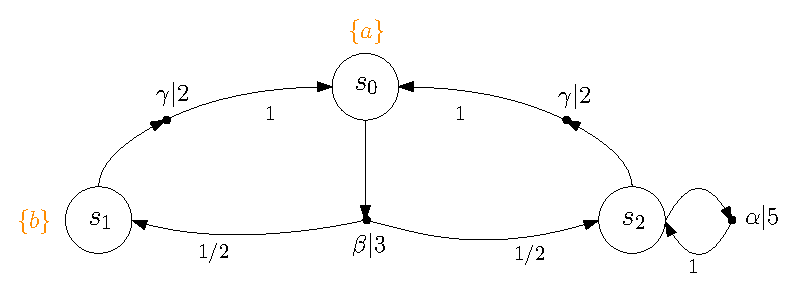
\includegraphics[width=\linewidth]{resources/simple-mdp}
    \captionsetup{justification=centering}
    \captionof{figure}{MDP $\mathcal{M}$, with $S = \{s_0, s_1, s_2\}$, $A = \{\alpha, \beta, \gamma\}$ and $AP = \{a, b\}$}\label{prism-simple}
\end{minipage}
\end{example}
